%\documentclass[aspectratio=169,handout]{beamer} % uncomment for handout mode
\documentclass[aspectratio=169]{beamer} % uncomment for presentation mode

\usepackage{style,amsmath, beamerthemesplit}
\setbeamertemplate{theorems}[numbered]
%\setbeameroption{show notes}% uncomment to see the notes

\title[Satz von Stone-Weierstraß]{Approximationssatz von Stone-Weierstraß}
\author{Pavel Zwerschke, Rafael Hirsch}
\date{17. Juli 2020}
\titlegraphic{
\includegraphics[scale=0.4]{kitlogo_de_rgb.pdf}}

\usetheme{berlin}

\begin{document}

\begin{frame}
    \maketitle
\end{frame}

\section{Approximationssatz von Weierstrass}

\frame{\frametitle{Approximationssatz von Weierstrass}
	\pause
	\begin{satz}
		Die Menge der Polynome liegt dicht in $C^0([a,b],\mathbb{R})$.
	\end{satz}
	\pause
	%\vspace{\baselineskip}
	Mit anderen Worten:
	\pause
	Für jedes $f\in C^0$ und jedes $\epsilon>0$ gibt es ein Polynom $p(x)$, sodass:\pause
	\begin{equation*}
		|f(x) - p(x)| < \epsilon
	\end{equation*}
	für alle $x\in[a,b]$.
	
	\pause
	\begin{block}{Bemerkung}
		Für den Beweis kann man oBdA annehmen, dass $[a,b] = [0,1]$. Ansonsten skaliert man $f$ einfach.
	\end{block}
}

\frame{\frametitle{Beweis 1}
	\pause
	Betrachten das n-te $Bernstein-Polynom:$
	\pause
	\begin{equation*}
		p_n(x) = \sum_{k=0}^n\binom{n}{k} c_kx^k(1-x)^{n-k},
	\end{equation*}
	wobei $c_k = f(\frac{k}{n})$. \\
	\ \\
	\pause
	Behauptung: $p_n(x)$ konvergiert gleichmäßig gegen $f$ für $n\to\infty$. \\
	\pause
	Dazu definieren wir:
	\begin{equation*}
		r_k(x) = \binom{n}{k} x^k(1-x)^{n-k} \pause\ge 0
	\end{equation*}
}

\frame{
	Für $r_k(x)$ gelten folgende Identitäten: \pause
	\begin{equation*}
		\sum_{k=0}^nr_k(x) = 1, \qquad \pause \sum_{k=0}^n(k-nx)^2r_k(x) = nx(1-x)
	\end{equation*}
	\pause
	Beweis kommt später. \pause
	 \\
	Damit gilt: \pause
	\begin{equation*}
		p_n(x) = \sum_{k=0}^nc_kr_k(x), \pause \qquad f(x)\pause =f(x)\sum_{k=0}^nr_k(x) 
		\pause =\sum_{k=0}^nf(x)r_k(x)
	\end{equation*}
	\pause

	$\Rightarrow p_n(x) - f(x)\pause =\sum_{k=0}^n(c_k-f(x))r_k(x)$
}

\frame{
	Sei $\epsilon>0$. \pause Wollen zeigen: \pause $|p_n(x) - f(x)| <\epsilon \quad \forall x\in[0,1]$ und n groß genug. \\
	\pause
	Da $f$ gleichmäßig stetig auf $[0,1]$, existiert $\delta>0$, sodass:
	\begin{align*}
		|t-s| <\delta \Rightarrow |f(t) - f(s)| < \frac{\epsilon}{2}
	\end{align*}
	\pause
	Definieren: \pause $K_1 = \left\{k\in \left\{0,...,n\right\}: |\frac{k}{n}-x|<\delta\right\}\quad$ \pause 
	und $\quad K_2 = \left\{0,...,n\right\}\setminus K_1.$\pause
	\begin{equation*}
		\begin{aligned}
			|p_n(x) - f(x)| \pause = \Big|\sum_{k=0}^n(c_k)-f(x))r_k(x)\Big| \pause\le\sum_{k=0}^n|c_k-f(x)|r_k(x) \\
			\pause = \sum_{k\in K_1}|c_k-f(x)|r_k(x) + \sum_{k\in K_2}|c_k-f(x)|r_k(x)
		\end{aligned}
	\end{equation*}
	\pause
	Werden beide Summen gegen $\frac{\epsilon}{2}$ abschätzen.
} 

\frame{
	\colorbox{yellow}{$\sum_{k\in K_1}|c_k-f(x)|r_k(x)$}\\
	\pause
	\ \\
	Es gilt: $|t-s| <\delta \Rightarrow |f(t) - f(s)| < \frac{\epsilon}{2}$ \pause
	\begin{equation*}
		\Rightarrow|c_k-f(x)| \pause = \Big|f\Big(\frac{k}{n}\Big)-f(x)\Big| \pause <\frac{\epsilon}{2} 
		\qquad\forall k\in K_1, \pause\qquad\Big(\Big|\frac{k}{n}-x\Big|<\delta \quad \forall k\in K_1\Big)
	\end{equation*}
	\pause
	Mit $\sum_{k=0}^nr_k(x) =1$ folgt: \pause
	\begin{equation*}
		\sum_{k\in K_1}|c_k-f(x)|r_k(x)\pause\le\sum_{k\in K_1}\frac{\epsilon}{2}r_k(x) 
		\pause\le\sum_{k=0}^n\frac{\epsilon}{2}r_k(x) \pause = \frac{\epsilon}{2}
	\end{equation*}
}

\frame{
	\colorbox{yellow}{$\sum_{k\in K_2}|c_k-f(x)|r_k(x)$}\\
	\ \\
	\pause
	Für $k\in K_2$ gilt:
	\begin{equation*}
		\Big|\frac{k}{n}-x\Big| \ge \delta \quad\pause\Leftrightarrow\quad 
		|k-nx|\ge n\delta \quad\pause\Leftrightarrow\quad (k-nx)^2\ge(n\delta)^2
	\end{equation*}
	\pause
	Mit der zweiten Identität von $r_k$ folgt: 
	\pause
	\begin{equation*}
		nx(1-x) = \sum_{k=0}^n(k-nx)^2r_k(x)\pause\ge \sum_{k\in K_2}(k-nx)^2r_k(x)
		\pause\ge \sum_{k\in K_2}(n\delta)^2r_k(x)
	\end{equation*}
	\pause
	Also:
	\begin{equation*}
		\sum_{k\in K_2}r_k(x) \pause\le \frac{nx(1-x)}{(n\delta)^2}\pause = \frac{x(1-x)}{n\delta^2}
	\end{equation*}
}

\frame{
	\colorbox{yellow}{$\sum_{k\in K_2}|c_k-f(x)|r_k(x)$}\\
	\ \\
	Es gilt: $x(1-x)\le\frac{1}{4} \quad\forall x\in[0,1].$ \pause Damit erhält man:
	\begin{equation*}
		\sum_{k\in K_2}r_k(x) \le \frac{x(1-x)}{n\delta^2}\pause\le\frac{1}{4n\delta^2}
	\end{equation*}
	\pause
	$|f|$ nimmt als stetige Funktion Maximum $M\in\mathbb{R}$ auf $[0,1]$ an.\pause
	\begin{equation*}
		\Rightarrow |c_k-f(x)|\le 2M \quad\forall x\in [0,1]
	\end{equation*}
	\pause
	Mit beiden Anschätzungen folgt für n groß genug:
	\pause
	\begin{equation*}
		\sum_{k\in K_2}|c_k-f(x)|r_k(x) \pause\le 2M\sum_{k\in K_2}r_k(x) 
		\pause\le \frac{M}{2n\delta^2} \pause\le \frac{\epsilon}{2}
	\end{equation*}
}

\frame{
	Bleiben noch die beiden Identitäten von $r_k$ zu zeigen. \\
	\pause
	Erinnerung:
	\begin{equation*}
		r_k(x) = \binom{n}{k}x^k(1-x)^{n-k}
	\end{equation*}
	\pause
	Betrachten binomischen Lehrsatz: $(x+y)^n = \sum_{k=0}^n\binom{n}{k}x^ky^{n-k}$ 
	\pause und setzen $y = 1-x$.
	\pause
	\begin{equation*}
		\Rightarrow \sum_{k=0}^nr_k(x) \pause = (x+(1-x))^n  \pause = 1
	\end{equation*}
	\pause
	Dies war gerade die erste Identität.
}

\frame{
	Zweite Identität: $\sum_{k=0}^n(k-nx)^2r_k(x) = nx(1-x).$ \\
	\pause
	Betrachten wieder binomischen Lehrsatz und leiten zweimal nach $x$ ab:
	\pause
	\begin{equation}
		n(x+y)^{n-1} = \sum_{k=0}^n \binom{n}{k}kx^{k-1}y^{n-k}
	\end{equation}
	\pause
	\begin{equation}
		n(n-1)(x+y)^{n-2} = \sum_{k=0}^n\binom{n}{k}k(k-1)x^{k-2}y^{n-k}
	\end{equation}
	\pause
	Setzen wieder $y=1-x$. \pause Multiplizieren (1) mit $x$ und (2) mit $x^2$:
	\pause
	\begin{equation}
		nx \pause = \sum_{k=0}^n\binom{n}{k}kx^k(1-x)^{n-k} \pause = \sum_{k=0}^nkr_k(x)
	\end{equation}
	\pause
	\begin{equation}
		n(n-1)x^2 \pause = \sum_{k=0}^n\binom{n}{k}k(k-1)x^k(1-x)^{n-k} \pause = \sum_{k=0}^nk(k-1)r_k(x)
	\end{equation}
}

\frame{
	$nx = \sum_{k=0}^nkr_k(x) \quad (3), \qquad n(n-1)x^2 = \sum_{k=0}^nk(k-1)r_k(x) \quad(4)$ \\
	\ \\
	\pause
	Umstellen von (4) und einsetzen von (3):
	\pause
	\begin{equation}
		\sum_{k=0}^nk^2r_k(x) \pause = n(n-1)x^2 + \sum_{k=0}^nkr_k(x) \pause = n(n-1)x^2 + nx
	\end{equation}
	\pause
	Aus (3), (5) und der ersten Identität folgt:
	\pause
	\begin{equation*}
		\begin{aligned}
			\sum_{k=0}^n(k-nx)^2r_k(x) \pause = \sum_{k=0}^nk^2r_k(x) - 2nx\sum_{k=0}^nkr_k(x) 
			+(nx)^2\sum_{k=0}^nr_k(x) \\
			\pause = n(n-1)x^2 + nx \pause - 2(nx)^2 \pause + (nx)^2 \pause = -nx^2 + nx \pause 
			= nx(1-x)
		\end{aligned}
	\end{equation*}
	\pause
	$\Rightarrow$ Zweite Identität\qed
}

\frame{\frametitle{Beweis 2}
	\pause
	Können Problem umformulieren: \\
	\pause
	Sei $g(x) = f(x) - (mx + b), \quad$ mit $m= f(1)-f(0)$ und $b = f(0)$ \\
	\pause
	$\Rightarrow g(0) = g(1) = 0$ \\
	\pause
	$\Rightarrow$ $g$ durch Polynome approximierbar $\Leftrightarrow$ f durch Polynome approximierbar\\
	\ \\
	\pause
	Sei also o.B.d.A $f(0) = f(1) = 0$ \pause und $f(x) = 0 \quad\forall x\in\mathbb{R}\setminus[0,1].$\\
	\pause
	$\Rightarrow$ $f$ stetig auf ganz $\mathbb{R}$\\
	\ \\
	\pause
	Betrachten Hilfsfunktion:
	\pause
	\begin{equation*}
		\beta_n(t) = b_n(1-t^2)^n\pause\ge0\quad -1\le t\le1,
	\end{equation*}
	\pause
	wobei $b_n$ so gewählt, dass $\int_{-1}^1\beta_n(t)\,dt = 1.$		
}

\frame{
	Definieren:
	\begin{equation*}
		P_n(x) := \int_{-1}^1f(x+t)\beta_n(t)\,dt \quad x\in[0,1]
	\end{equation*}
	\pause
	Behauptung: $P_n$ ist Polynom und konvergiert gleichmäßig gegen $f$.\\
	\pause
	Substituieren mit $u = x+t$:
	\pause
	\begin{equation*}
		\Rightarrow P_n(x) = \int_{x-1}^{x+1}f(u)\beta_n(u-x)\,du \pause = \int_0^1f(u)\beta_n(u-x)\,du
	\end{equation*}
	da $f=0$ außerhalb von $[0,1]$\\
	\pause
	\ \\
	$\beta_n$ ist Polynom $\pause\Rightarrow$ können Potenzen von $x$ mit Linearität aus Integral ziehen \\ 
	\pause $\Rightarrow$ $P_n(x)$ ist Polynom. 
}

\frame{
	Zeigen zuerst:\\
	\pause
	Sei $\delta>0 \Rightarrow\beta_n(t)$ konvergiert gleichmäßig gegen $0$ für $\delta\le|t|\le1.$\\
	\ \\
	\pause
	Erinnerung: $\beta_n(t) = b_n(1-t^2)^n$.\\
	\pause
	Es gilt:
	\begin{equation*}
		1 = \int_{-1}^1\beta_n(t)\,dt \pause\ge \int_{\frac{-1}{\sqrt{n}}}^{\frac{1}{\sqrt{n}}}b_n(1-t^2)^n\,dt
		\pause\ge \int_{\frac{-1}{\sqrt{n}}}^{\frac{1}{\sqrt{n}}}b_n(1-\frac{1}{n})^n\,dt 
		\pause= b_n\frac{2}{\sqrt{n}}(1-\frac{1}{n})^n
	\end{equation*}
	\pause
	Da $(1-\frac{1}{n})^n$ beschränkt, gilt:
	\pause
	\begin{equation*}
		b_n\le(1-\frac{1}{n})^{-n}\frac{\sqrt{n}}{2}\pause\le c\sqrt{n}
	\end{equation*}	
	für eine Konstante $c\in \mathbb{R}$ und alle $n\ge2$.
}

\frame{
	$b_n\le c\sqrt{n}$\\
	\pause
	Daraus folgt für $\delta\le|t|\le1$:
	\pause
	\begin{equation*}
		\beta_n(t) = b_n(1-t^2)^n\pause\le c\sqrt{n}(1-t^2)^n\pause\le c\sqrt{n}(1-\delta^2)^n
		\pause\to 0\qquad (n\to\infty)
	\end{equation*}
	\pause
	$\Rightarrow \beta_n\to 0$ gleichmäßig auf $\delta\le|t|\le1$. \\
	\pause \ \\
	Zeigen nun: $P_n\to f$ gleichm\"aßig.\\
}

\frame{
	Sei $\epsilon>0$. \pause Da $f$ gleichm\"aßig stetig auf $[0,1]$ existiert $\delta>0$, sodass:
	\begin{equation*}
		|t|<\delta\Rightarrow |f(x+t) - f(x)|<\frac{\epsilon}{2}.
	\end{equation*}
	\pause
	Erinnerung: $\int_{-1}^1\beta_n(t)\,dt = 1$
	\pause 
	\begin{equation*}
		\begin{aligned}|P_n(x) - f(x)| \pause= \bigg|\int_{-1}^1f(x+t)\beta_n(t)\,dt -f(x)\bigg| \\
			\pause
			= \bigg|\int_{-1}^1(f(x+t)-f(x))\beta_n(t)\,dt\bigg| \pause\le\int_{-1}^1|f(x+t)-f(x)|\beta_n(t)\,dt \\ 
			\pause
			= \int_{|t|<\delta}|f(x+t)-f(x)|\beta_n(t)\,dt + \int_{|t|\ge\delta}|f(x+t)-f(x)|\beta_n(t)\,dt \\
			\pause
			\le \frac{\epsilon}{2} \pause+ \int_{|t|\ge\delta}|f(x+t)-f(x)|\beta_n(t)\,dt
		\end{aligned}
	\end{equation*}
}	

\frame{
	\colorbox{yellow}{$\int_{|t|\ge\delta}|f(x+t)-f(x)|\beta_n(t)\,dt$}\\
	\ \\
	\pause
	Sei $M\in\mathbb{R}$ das Maximum von $|f|$ auf $[0,1]$.\\
	\pause
	Wissen: $\beta_n(t)$ konvergiert gleichmäßig gegen $0$ für $\delta\le|t|\le1$.
	\pause
	\begin{equation*}
		\Rightarrow \int_{|t|\ge\delta}|f(x+t)-f(x)|\beta_n(t)\,dt \pause\le 2M\int_{|t|\ge\delta}\beta_n(t)\,dt
		\pause\le \frac{\epsilon}{2}
	\end{equation*}
	für n groß genug.
	\qed
}

\section{Approximationssatz von Stone-Weierstraß}

\begin{frame}{Funktionenalgebra}
    \begin{defi}[Funktionenalgebra]
        Eine Menge \( \mathcal{A} \subset \mathcal{C}^0(M) \) heißt 
        \textit{Funktionenalgebra}, wenn sie abgeschlossen unter Addition, 
        skalarer Multiplikation und Funktionenmultiplikation ist, 
        d.~h. \( \forall f,g \in \A, c \in \mathbb{R} \)
        \[ f + g \in \mathcal{A}, \quad c \cdot f \in \mathcal{A}, \quad f \cdot g \in \mathcal{A}. \]
    \end{defi}
\end{frame}

\begin{frame}{Verschwinden}
    \begin{defi}[Verschwinden]
        Eine Funktionenalgebra \(\A \subset \CM\) 
        \textit{verschwindet} an einem Punkt \(p \in M\), falls 
        \[ f(p) = 0 \;\forall f \in \mathcal{A}. \]
    \end{defi}
    \pause
    \begin{bsp}
        \( \A := \set{ x \mapsto \sum_{j=1}^n a_n x^n \;|\; n\in \N, a_j \in \R, j = 1,\ldots, n } \subset \mathcal{C}^0([-1,1]) \) 
        verschwindet im Punkt \(0\).
    \end{bsp}
\end{frame}

\begin{frame}{Punktetrennend}
    \begin{defi}
        Eine Funktionenalgebra \(\A \subset \CM\) ist \textit{punktetrennend}, 
        wenn für beliebige \( p_1, p_2 \in M \), \(p_1 \neq p_2\), 
        eine Funktion \(f \in \A\) existiert, 
        sodass \( f(p_1) \neq f(p_2) \).
    \end{defi}
    \pause
    \begin{bsp}
        \( \A := \set{ x \mapsto \sum_{j=0}^n a_{j} x^{2j} \;|\; n\in\N, a_j \in \R, j = 1,\ldots, n } 
        \subset \mathcal{C}^0([-1,1]) \)
        trennt die Punkte \( z \) und \(-z\) (\(z \in [-1,1] \setminus \set{0} \)) nicht, da \( \forall f \in \A \) gilt 
        \( f(z) = f(-z) \).
    \end{bsp}
    \pause
    \begin{bsp}
        Die Funktionenalgebra aller trigonometrischen Polynome auf \( [0,2\pi) \) 
        \(\mathcal{T} = \set{x \mapsto T(x) = a_0 + \sum_{k=1}^n a_k \cos(kx) + \sum_{k=1}^n b_k \sin(kx)}\) 
        trennt Punkte und verschwindet nirgends.
    \end{bsp}
\end{frame}

\begin{frame}{Satz von Stone-Weierstraß}
    \begin{satz}[Satz von Stone-Weierstraß]
        Sei \(M\) ein kompakter metrischer Raum und \( \mathcal{A} \) eine punktetrennende
        Funktionenalgebra in \( \mathcal{C}^0(M) \), die nirgends verschwindet. 
        Dann ist \( \mathcal{A} \) dicht in \( \mathcal{C}^0(M) \).
    \end{satz}
    \pause
    \begin{bem}
        Der Satz von Stone-Weierstraß ist offensichtlich eine Verallgemeinerung 
        des Satzes von Weierstraß. 
        Wir benötigen die Aussage des Satzes von Weierstraß für den Beweis von Stone-Weierstraß.
    \end{bem}
\end{frame}

\begin{frame}
    \begin{lem}\label{bel-punkte}
        Sei \( \A \subset \CM \) eine punktetrennende Funktionenalgebra, die nirgends verschwindet. 
        Dann existiert für beliebige \( p_1, p_2 \in M, p_1\neq p_2, 
        c_1, c_2 \in \R \)
        ein \(f \in \A\) mit 
        \[ f(p_1) = c_1, \quad f(p_2) = c_2. \]
    \end{lem}
\end{frame}

\begin{frame}{Beweis von Lemma \ref{bel-punkte}}
    Seien \( p_1, p_2 \in M \) und \( c_1, c_2 \in \R \) gegeben. 
    \pause

    Da \(\A\) nirgends verschwindet, existieren \( g_1, g_2 \in \A \), 
    sodass 
    \( g_1(p_1) \neq 0, g_2(p_2) \neq 0 \). 
    \pause

    Also gilt \( g := g_1^2 + g_2^2 \in \A \). \(g\) verschwindet weder in \(p_1\) noch \(p_2\).
    \pause 

    \(\A\) trennt Punkte, also existiert ein \( h \in \A \), sodass 
    \( h(p_1) \neq h(p_2) \).
    \pause 
    Betrachten wir die Matrix 

    \[ H = \begin{pmatrix}
        a & ab \\
        c & cd
    \end{pmatrix} = \begin{pmatrix}
        g(p_1) & g(p_1) h(p_1) \\
        g(p_2) & g(p_2) h(p_2)
    \end{pmatrix}. \]
    \pause

    Nach Konstruktion gilt 
    \( a, c \neq 0 \) sowie \(b \neq d\). Also gilt \( \det H = acd - abc = ac(d - b) \neq 0 \). 
\end{frame}

\begin{frame}
    Somit hat das LGS 
    \begin{align*}
        a \xi + ab \eta &= c_1 \\
        c \xi + cd \eta &= c_2
    \end{align*}

    genau eine Lösung für \( \xi \) und \( \eta \). 
    \pause
    Sei \( f := \xi g + \eta g h \). \pause 
    Offensichtlich ist \( f \in \A \) \pause 
    und es gilt 
    \begin{align*}
        f(p_1) &= \xi g(p_1) + \eta g(p_1) h(p_1) = c_1, \\
        f(p_2) &= \xi g(p_2) + \eta g(p_2) h(p_2) = c_2.
    \end{align*}
    \qed
\end{frame}

\begin{frame}
    \begin{lem}\label{abg-algebra}
        Sei \( \A \subset \CM \) eine Funktionenalgebra 
        sowie \(M\) ein kompakter metrischer Raum.
        Dann ist \( \Abar \) ebenfalls eine Funktionenalgebra.
    \end{lem} \pause
    Beweis: \pause 
    Stimmt so. \qed
\end{frame}

\begin{frame}
    \begin{lem}\label{betrag-in-algebra}
        Sei \( \A \subset \CM \) eine Funktionenalgebra. Dann gilt 
        \[ f \in \Abar \Rightarrow \abs{f} \in \Abar \]
        sowie 
        \[ f_1, \ldots, f_n \in \Abar \Rightarrow \max(f_1,\ldots, f_n), \min(f_1,\ldots, f_n) \in \Abar. \]
    \end{lem} \pause
    Beweis:
    Nach dem Satz von Weierstraß existiert ein Polynom 
    \( p(y) \), sodass 
    \[ \sup \set{ \abs{ p(y) - \abs{y} } 
    \;|\; \abs{y} \leq \norm{f} } < \frac{\varepsilon}{2}, \]
    da \( \abs{y} \in \C([-\norm{f}, \norm{f}]) \). 
    \pause

    Der konstante Term dieses Polynoms ist höchstens \( \varepsilon / 2 \), 
    da \( \abs{ p(0) - \abs{0} } < \varepsilon/2 \).
\end{frame}

\begin{frame}
    Sei \( q := p - p(0) \). Dann ist \( q(y) \) ein 
    Polynom mit Konstante \(0\) und es gilt 
    \[ \abs{ q(y) - \abs{y} } < \varepsilon 
    \;\forall y \in [-\norm{f}, \norm{f}]. \]
    \pause

    Wir schreiben \( q \) nun als 
    \( q(y) = a_1 y + a_2 y^2 + \cdots + a_n y^n \) und 
    \[ g = a_1 f + a_2 f^2 + \cdots + a_n f^n. \]
    \pause

    \( \Abar \) ist eine Funktionenalgebra (Lemma \ref{abg-algebra}).
    Somit gilt \( g \in \Abar \). 
    \pause

    Sei \( x\in M \) und \( y = f(x) \). Dann gilt 
    \[ \abs{ g(x) - \abs{f(x)} } = \abs{ q(y) - \abs{y} } < \varepsilon. \]
    \pause
    
    Also folgt \( \abs{f} \in \Abarbar = \Abar \). 
\end{frame}

\begin{frame}
    Außerdem gilt, falls \(f,g \in \Abar \)
    \pause
    \begin{align*}
        \max(f,g) &= \frac{f+g}{2} + \frac{\abs{f-g}}{2}, \\
        \min(f,g) &= \frac{f+g}{2} - \frac{\abs{f-g}}{2}.
    \end{align*} 
    \pause
    Also gilt \( \max(f,g), \min(f,g) \in \Abar \). 
    \pause

    Mittels Induktion können wir dies für beliebige endliche
    \( f_1, \ldots, f_n \in \Abar \) fortführen.
    \qed
\end{frame}

\begin{frame}{Beweis vom Satz von Stone-Weierstraß}
    Sei \( \A \) eine punktetrennende Funktionenalgebra in \(\CM\), die nirgends verschwindet. \pause
    Wir zeigen nun, dass \( \A \) dicht in \(\CM\) ist. \pause
    D. h. für ein gegebenes \( F \in \CM, \varepsilon > 0 \) 
    müssen wir ein \( G \in \A \) finden, sodass 
    \[ F(x) - \varepsilon < G(x) < F(x) + \varepsilon. \]
    \pause

    Wir betrachten nun zwei Punkte \(p\neq q \in M\).
    Nach Lemma \ref{bel-punkte} existiert ein \(H_{pq} \in \A\), 
    sodass 
    \[ H_{pq}(p) = F(p), \quad H_{pq}(q) = F(q). \]
\end{frame}

\begin{frame}
    \begin{columns}
        \begin{column}{0.4\textwidth}
            Wir fixieren nun \(p\).
            \onslide<2->{Für jedes \(q \in M\) existiert eine Umgebung 
            \( U_q \)}\onslide<3->{, sodass 
            \[ x \in U_q \Rightarrow F(x) - \varepsilon < H_{pq}(x). \]}
            % H_{pq} ist stetig
        \end{column}
        \begin{column}{0.6\textwidth}
            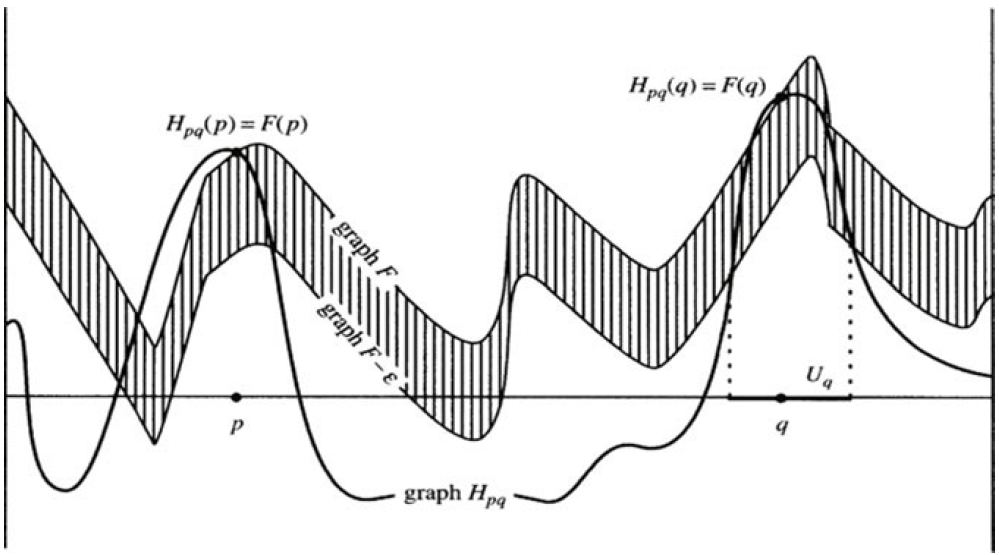
\includegraphics[width=\textwidth]{images/stone-weierstrass-step1.png}
        \end{column}
    \end{columns}
\end{frame}

\begin{frame}
    \cbox{Überdeckungskompakt: Für beliebige Überdeckung \( M = \bigcup_{i\in I} U_i \) 
    existiert eine endliche Indexmenge \(J \subset I\), 
    sodass \(M = \bigcup_{j\in J} U_j\) ist.}\vspace{0.5em} \\ 

    \begin{columns}
        \begin{column}{0.4\textwidth}
            \( M \) ist kompakt \( \Rightarrow \) endlich viele 
            \( U_{q_1}, \ldots, U_{q_n} \) überdecken \(M\).
            \onslide<2->{Sei 
            \[ G_p := \max(H_{pq_1}, \ldots, H_{pq_n}). \]}
            
            \onslide<4->{Nach Lemma \ref{betrag-in-algebra} gilt \( G_p \in \Abar \).}
            \onslide<5->{Es gilt nun \(G_p(p) = F(p)\)} \onslide<6->{sowie \( \forall x \in M \)
            \[ F(x) - \varepsilon < G_p(x). \]}
        \end{column}
        \begin{column}{0.6\textwidth}
            \onslide<3->{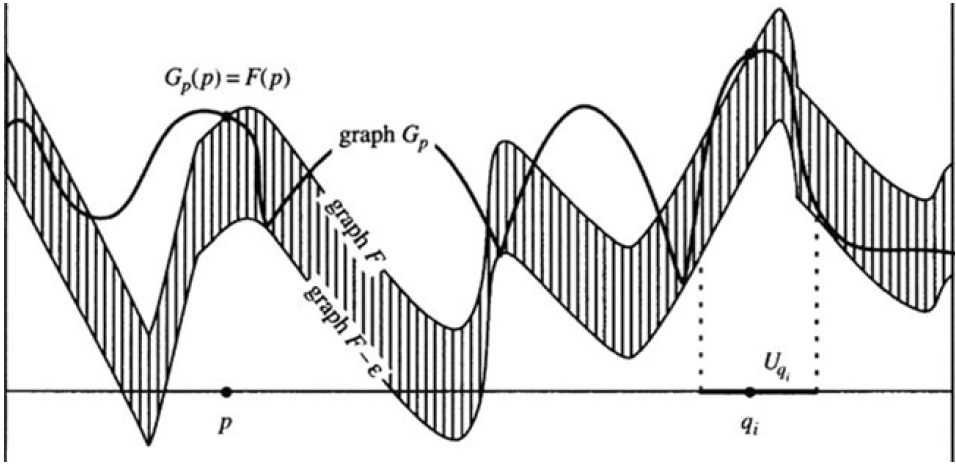
\includegraphics[width=\textwidth]{images/stone-weierstrass-step2.png}}
        \end{column}
    \end{columns}
\end{frame}

\begin{frame}
    \begin{columns}
        \begin{column}{0.4\textwidth}
            Sei nun \(p\) variabel.
            \onslide<2->{\(G_p\) stetig}
            \onslide<3->{\( \Rightarrow \forall p \in M \;\exists V_p: \)
            \[ x \in V_p \Rightarrow G_p(x) < F(x) + \varepsilon. \]}

            \onslide<5->{Nun folgt wieder aus der Kompaktheit von \(M\), dass 
            endlich viele \( V_{p_1}, \ldots, V_{p_m} \) \(M\) überdecken.}
        \end{column}
        \begin{column}{0.6\textwidth}
            \onslide<4->{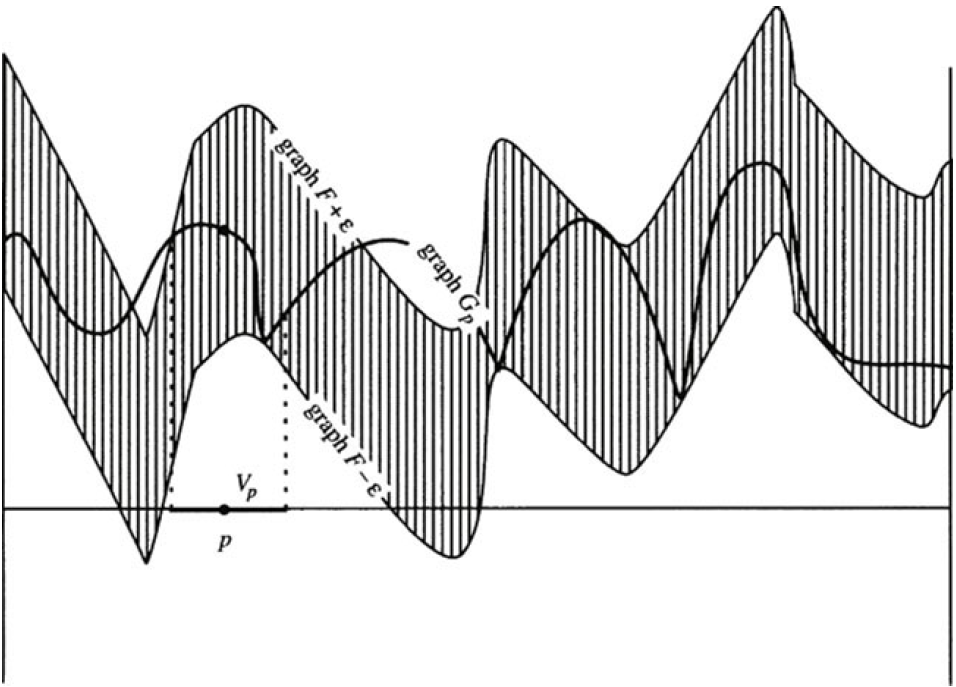
\includegraphics[width=\textwidth]{images/stone-weierstrass-step3.png}}
        \end{column}
    \end{columns}
\end{frame}

\begin{frame}
    \begin{columns}
        \begin{column}{0.4\textwidth}
            Sei \( G := \min(G_{p_1}, \ldots, G_{p_m}) \).

            \onslide<3->{Es folgt nun aus Lemma \ref{betrag-in-algebra}
            \( G \in \Abar \)} \onslide<4->{sowie 
            \[ F(x) - \varepsilon < G(x) < F(x) + \varepsilon \;\forall x \in M. \]}

            \onslide<5->{Also liegt \( \Abar \) dicht in \( \CM \)}\onslide<6->{, d. h. \( \Abar = \Abarbar = \CM \).}

            \onslide<7->{Also liegt auch \( \A \) dicht in \(\CM\).
            \qed}
        \end{column}
        \begin{column}{0.6\textwidth}
            \onslide<2->{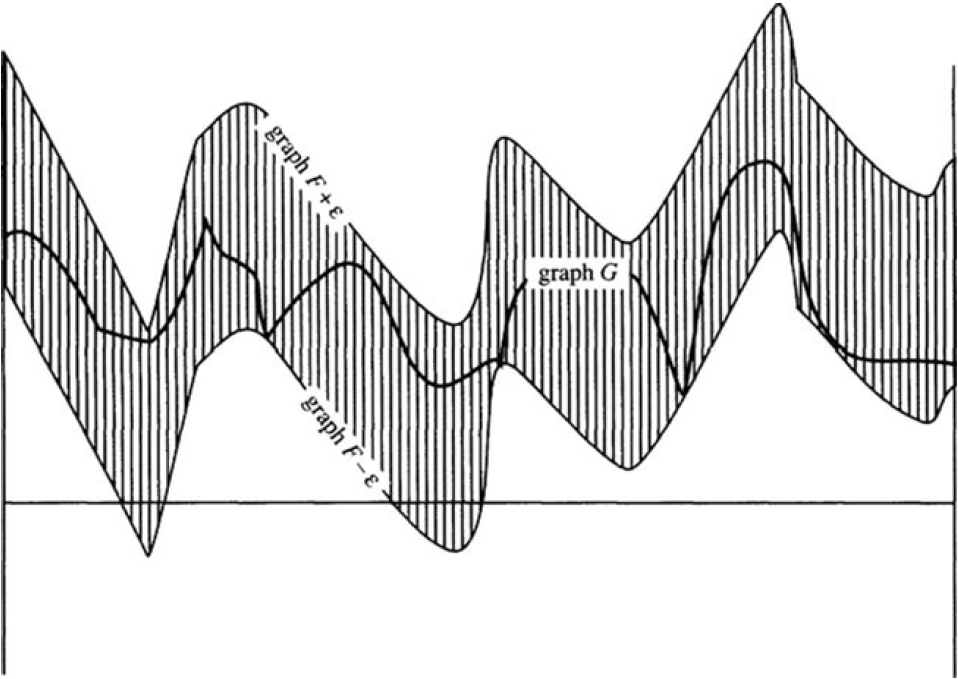
\includegraphics[width=\textwidth]{images/stone-weierstrass-step4.png}}
        \end{column}
    \end{columns}
\end{frame}

\section*{Anwendungen von Stone-Weierstraß}

\begin{frame}
    \begin{satz}
        Jede \(2\pi\)-periodische stetige Funktion kann gleichmäßig durch ein trigonometrisches Polynom 
        \[ T(x) = a_0 + \sum_{k=1}^n a_k \cos(kx) + \sum_{k=1}^n b_k \sin(kx) \]
        approximiert werden.
    \end{satz}
    \pause
    Beweis:
    \( [0,2\pi) \) parametrisiert den Einheitskreis \(S^1\) durch \( x \mapsto (\cos x, \sin x) \). 
    \pause
    \(S^1\) ist kompakt und jede \(2\pi\)-periodische Funktion auf \(\R\) wird hier zu einer 
    stetigen Funktion auf \(S^1\).
    \pause

    Die trigonometrischen Polynome bilden eine Funktionenalgebra \( \mathcal{T} \subset \C(S^1) \), 
    die \textit{nirgends verschwindet} und \textit{Punkte trennt}.
    \pause

    Nach dem Satz von Stone-Weierstraß liegt \( \mathcal{T} \) dicht in \( \C(S^1) \). \qed
\end{frame}

\newcommand{\B}{\overline{B_1(0)}}

\begin{frame}{Vektorfelder}
    Betrachten wir ein stetiges Vektorfeld 
    \( \abb{F}{\B}{\R^2} \).\pause

    Wir wollen \( F \) durch ein Vektorfeld, das maximal endlich 
    häufig verschwindet, approximieren.
    \pause

    Betrachte die Funktionenalgebra \( \A \subset \C(\B) \) 
    der reellen Polynome in zwei Variablen \pause
    \[ \A = \set{ x \mapsto \sum_{i,j=0}^n c_{ij} x^i y^j \;|\; c_{ij} \in \R }. \]
    \pause

    Dies ist eine Algebra, die \textit{nirgends verschwindet} und \textit{Punkte trennt}.
    \pause

    Aus dem Satz von Stone-Weierstraß folgt, dass \(\A\) dicht in \( \C(\B) \) ist 
    und so können wir \( F = (F_1, F_2) \) durch Polynome 
    \( F_1 \approx P, F_2 \approx Q \) approximieren.
\end{frame}

\end{document}
